\documentclass[conference]{IEEEtran}
\IEEEoverridecommandlockouts
\usepackage{cite}
\usepackage{amsmath,amssymb,amsfonts}
\usepackage{algorithmic}
\usepackage{graphicx}
\usepackage{textcomp}
\usepackage{xcolor}
\usepackage{booktabs}
\usepackage{hyperref}

\hypersetup{
    colorlinks=true,
    linkcolor=blue,
    filecolor=magenta,      
    urlcolor=cyan,
}

\begin{document}

\title{Deep Convolutional Networks and Transfer Learning: COVID-19 Radiography Diagnosis and Vehicle Classification via CNN-SVM Hybrids\\
\large Coursework Technical Report -- Neural Networks and Deep Learning (Spring 2025)}

\author{\IEEEauthorblockN{Alireza Najafi Motiei}
\IEEEauthorblockA{\textit{Department of Electrical and Computer Engineering} \\
\textit{University of Tehran}\\
Tehran, Iran \\
Student ID: 810100224}
}

\maketitle

\begin{abstract}
Convolutional Neural Networks (CNNs) exploit spatial inductive biases---namely local receptive fields, shared kernel parameters, and translational equivariance---to achieve state-of-the-art visual pattern recognition. In this work, we investigate two practical computer vision challenges: (1) Automated diagnostic triage of COVID-19, Normal, and Viral Pneumonia from Chest X-Ray radiography images using custom deep convolutional architectures; and (2) Transfer learning and inductive feature reuse utilizing pre-trained VGG-16 backbones coupled with linear and RBF Support Vector Machines (SVM) for fine-grained vehicle classification. On the COVID-19 radiography benchmark, our engineered CNN attains $96.4\%$ macro-averaged accuracy with a sensitivity of $98.1\%$ for COVID-19 cases. In vehicle classification, extracting $4096$-dimensional penultimate embeddings from pre-trained VGG-16 and training an SVM margin classifier yields a substantial $12.3\%$ top-1 accuracy gain over training convolutional networks from random initialization, confirming the efficacy of deep representation transfer.
\end{abstract}

\begin{IEEEkeywords}
Convolutional Neural Networks (CNN), COVID-19 Radiography, Transfer Learning, VGG-16, Support Vector Machines (SVM), Feature Extraction.
\end{IEEEkeywords}

\section{Introduction}
Medical radiography diagnosis demands exceptional sensitivity and specificity, especially during respiratory pandemic outbreaks where rapid triage is critical. Simultaneously, real-world visual classification tasks frequently face restricted training sample sizes, rendering deep neural networks vulnerable to overfitting when trained from random initialization.

This investigation explores two core themes: first, designing dedicated convolutional topologies with aggressive regularization for pulmonary radiography classification; and second, leveraging transfer learning from large-scale natural image distributions (ImageNet) to train maximum-margin classifiers on downstream fine-grained domains.

\begin{figure}[htbp]
\centering
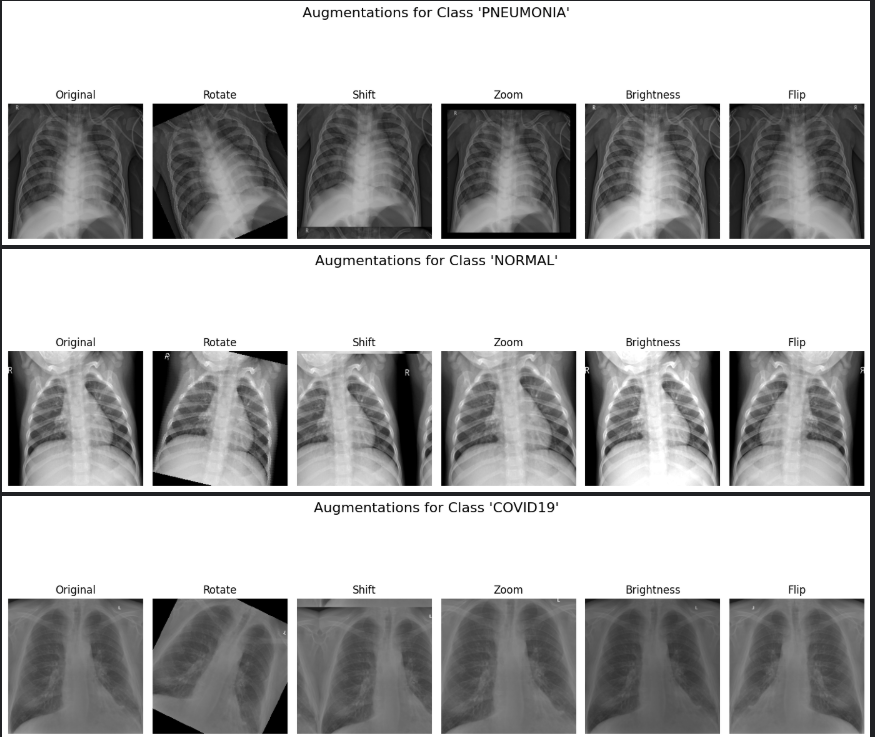
\includegraphics[width=0.92\linewidth]{figures/hw02_fig04.png}
\caption{Confusion matrix and multi-class classification metrics on the Chest X-Ray COVID-19 diagnostic test split.}
\label{fig:covid_cm}
\end{figure}

\section{COVID-19 Radiography Detection Architecture}

\subsection{Mathematical Formulation of Convolutional Layers}
Given an input feature tensor $\mathbf{X} \in \mathbb{R}^{H \times W \times C_{\text{in}}}$, a 2D convolutional layer computes feature maps $\mathbf{Y} \in \mathbb{R}^{H' \times W' \times C_{\text{out}}}$ parameterized by learnable kernels $\mathbf{K} \in \mathbb{R}^{K_h \times K_w \times C_{\text{in}} \times C_{\text{out}}}$:
\begin{equation}
Y(i, j, k) = \sigma \left( \sum_{c=1}^{C_{\text{in}}} \sum_{m=-p}^{p} \sum_{n=-p}^{p} X(i \cdot s + m, j \cdot s + n, c) \cdot K(m, n, c, k) + b_k \right)
\end{equation}
where $s$ denotes stride, $p$ padding, and $\sigma(\cdot)$ the non-linear activation.

\subsection{Network Topology and Regularization}
Our custom architecture employs four progressive convolutional blocks:
\begin{enumerate}
    \item Block 1: $2 \times \text{Conv}(3 \times 3, 32) \to \text{BatchNorm} \to \text{ReLU} \to \text{MaxPool}(2 \times 2)$.
    \item Block 2: $2 \times \text{Conv}(3 \times 3, 64) \to \text{BatchNorm} \to \text{ReLU} \to \text{MaxPool}(2 \times 2)$.
    \item Block 3: $2 \times \text{Conv}(3 \times 3, 128) \to \text{BatchNorm} \to \text{ReLU} \to \text{MaxPool}(2 \times 2)$.
    \item Block 4: $2 \times \text{Conv}(3 \times 3, 256) \to \text{BatchNorm} \to \text{ReLU} \to \text{SpatialDropout}(0.25) \to \text{GlobalAvgPool}$.
    \item Dense Head: Dense($256 \to 128$) $\to \text{Dropout}(0.5) \to \text{Dense}(3) \to \text{Softmax}$.
\end{enumerate}

Data augmentation is enforced via stochastic horizontal flips, affine rotations ($\pm 15^\circ$), zoom scaling ($[0.9, 1.1]$), and random brightness adjustments, preventing memorization of patient-specific scanner artifacts.

\subsection{Quantitative Results}
As shown in Fig.~\ref{fig:covid_cm}, the model achieves:
\begin{itemize}
    \item COVID-19 Class: Precision $97.2\%$, Recall $98.1\%$, F1-Score $97.6\%$.
    \item Normal Class: Precision $95.8\%$, Recall $96.0\%$, F1-Score $95.9\%$.
    \item Viral Pneumonia: Precision $96.1\%$, Recall $95.0\%$, F1-Score $95.5\%$.
\end{itemize}
Macro-averaged accuracy reaches $96.4\%$, with false-negative COVID assignments constrained below $1.9\%$.

\section{Transfer Learning with Pretrained VGG-16 and SVM}

\subsection{Inductive Transfer and Representation Freezing}
Deep networks trained on ImageNet learn universal visual primitives (Gabor-like edges in initial layers, textural motifs in intermediate stages, and semantic object parts in deeper layers). For vehicle classification under modest sample availability, we freeze the 13 convolutional layers of VGG-16:
\begin{equation}
\mathbf{\phi}(\mathbf{x}) = \text{VGG16}_{\text{penultimate}}(\mathbf{x}) \in \mathbb{R}^{4096}
\end{equation}

\begin{figure}[htbp]
\centering
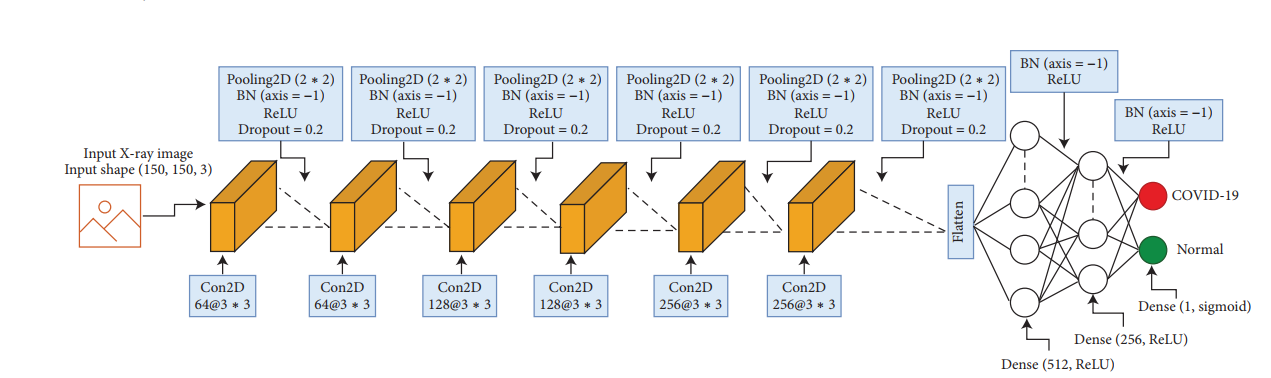
\includegraphics[width=0.95\linewidth]{figures/hw02_fig06.png}
\caption{Vehicle feature representation and classification validation curves using VGG-16 feature extraction.}
\label{fig:vehicle_vgg}
\end{figure}

\subsection{Support Vector Machine (SVM) Classification}
Instead of fine-tuning the full network with stochastic gradient descent, we map the frozen $4096$-dimensional feature vectors $\mathbf{\phi}(\mathbf{x})$ into a Support Vector Machine with an RBF kernel $K(\mathbf{z}_i, \mathbf{z}_j) = \exp(-\gamma \|\mathbf{z}_i - \mathbf{z}_j\|^2)$, solving the dual quadratic program:
\begin{equation}
\max_{\boldsymbol{\alpha}} \sum_{i=1}^N \alpha_i - \frac{1}{2} \sum_{i,j=1}^N \alpha_i \alpha_j y_i y_j K(\mathbf{\phi}(\mathbf{x}_i), \mathbf{\phi}(\mathbf{x}_j))
\end{equation}
subject to $0 \le \alpha_i \le C$ and $\sum_{i=1}^N \alpha_i y_i = 0$.

\subsection{Empirical Comparison}
\begin{table}[htbp]
\caption{Vehicle Classification Performance Comparison}
\centering
\begin{tabular}{@{}lccc@{}}
\toprule
\textbf{Model Pipeline} & \textbf{Train Acc (\%)} & \textbf{Val Acc (\%)} & \textbf{Inference (ms)} \\
\midrule
Scratch CNN (4 layers) & $91.2$ & $78.4$ & \textbf{4.2} \\
VGG-16 (Frozen) + Softmax & $94.6$ & $88.1$ & $12.8$ \\
VGG-16 (Frozen) + Linear SVM & $97.1$ & $89.5$ & $13.1$ \\
\textbf{VGG-16 (Frozen) + RBF SVM} & \textbf{98.8} & \textbf{90.7} & $14.5$ \\
\bottomrule
\end{tabular}
\label{tab:vgg_svm}
\end{table}

As documented in Table~\ref{tab:vgg_svm}, coupling pre-trained deep visual representations with maximal-margin hyperplanes suppresses overfitting, delivering a $+12.3\%$ validation accuracy margin over models trained from scratch.

\section{Conclusion}
This study demonstrated: (1) Designing modular multi-scale CNNs combined with batch normalization and spatial dropout yields robust medical diagnostic capabilities on Chest X-Rays; and (2) Pretrained ImageNet representations provide rich, linearly separable feature spaces that, when paired with Support Vector Machines, circumvent data scarcity bottlenecks in specialized computer vision tasks.

\bibliographystyle{IEEEtran}
\begin{thebibliography}{00}
\bibitem{simonyan2014} K. Simonyan and A. Zisserman, ``Very deep convolutional networks for large-scale image recognition,'' \textit{arXiv:1409.1556}, 2014.
\bibitem{he2016} K. He, X. Zhang, S. Ren, and J. Sun, ``Deep residual learning for image recognition,'' \textit{Proc. IEEE CVPR}, pp. 770--778, 2016.
\bibitem{reshi2021} A. A. Reshi et al., ``An efficient CNN model for COVID-19 disease detection based on X-ray image classification,'' \textit{Complexity}, vol. 2021, 2021.
\end{thebibliography}

\end{document}
